% 阶段报告四：中文正式版。编译：xelatex stage_report_4_zh.tex（两遍）。
% 数字来源及独立核验见本目录 verified_numbers.json 和 README.md。
\documentclass[11pt,a4paper,UTF8,fontset=fandol]{ctexart}
\usepackage[margin=0.9in]{geometry}
\usepackage{amsmath,amssymb,booktabs,tabularx,array,graphicx,xcolor,float}
\usepackage[hidelinks]{hyperref}
\usepackage{enumitem}
\setlist{itemsep=3pt,topsep=5pt}
\renewcommand{\refname}{参考文献}
\newcolumntype{Y}{>{\raggedright\arraybackslash}X}
\newcommand{\code}[1]{\nolinkurl{#1}}
\emergencystretch=3em
\linespread{1.15}
\setlength{\parindent}{2em}
\setlength{\parskip}{0pt}
% 页眉沿用 ctexart 默认 headings 样式，但保留节标题原大小写（E2a 不被大写为 E2A）。
\makeatletter
\renewcommand\sectionmark[1]{\markboth{\ifnum\c@secnumdepth>\z@\thesection\quad\fi #1}{}}
\makeatother
\title{\bfseries 两倍尺度为何改善 Dead 检测：机制对照、专家分支检验与推理成本\\[7pt]
\large PanNuke 细胞核实例分割：阶段报告四}
\author{课程项目 bdd26}
\date{2026 年 10 月 8 日\\\small 实验范围：2026 年 10 月 6 日至 8 日；10 月 9 日勘误，10 月 10 日文字修订}
\begin{document}
\maketitle

\begin{abstract}
上一阶段，EF-P2 在保留原尺度预测的基础上，筛选并补入两倍尺度模型独有的候选核，取得了小幅 Dead PQ 增益。但这一结果留下了三个问题：增益来自哪里，能否通过模型内的 Dead 专家分支获得，以及两套模型需要付出多少推理成本。本阶段分别检验这三个问题。四组对照实验（E2a）比较了工作尺度与 HV 目标面积门槛：在原尺度上降低门槛，所获 Dead PQ 增益仅为原两倍尺度增益的 9.59\%；把门槛换算到原图面积后再比较，两倍尺度仍表现为官方 Dead PQ 均值上升、bPQ 下降，且 strict Dead 在四组配对比较中均下降。Dead 专家分支（DSB）则按事先登记的四项条件决定是否启动训练。梯度探针在修正取样后发现，训练完成的基线模型上，64 个有效批次的解码器复合梯度余弦均值为 $+0.749$、最小值为 $+0.594$，没有负值，不支持本方案预设的梯度冲突前提。因此，DSB 按预注册规则停止，未训练专家分支。推理计时显示，两模型系统约需单模型 x1 的 6.1 倍时间；10 月 9 日用同一份计时记录修正加权方式后，比值为 6.08447，并非一次新测量。EF-P2 因而保留为机制分析和后续教师模型的候选，不作为已有部署优势。E2a、DSB、E0 的新实验仅使用训练折和验证折；另行开展的审计核查了历史测试产物，没有新增三划分测试成绩。
\end{abstract}
\noindent\textbf{关键词：}细胞核实例分割；PanNuke；尺度对照；预注册检验；梯度冲突；推理成本

\section{研究背景与本阶段问题}

阶段报告三显示，EF-P2 在九组划分--种子配对上将 Dead PQ 平均提高 0.00699，bPQ 的平均变化约为 $-0.000009$\cite{reports}。它通过了事先规定的联合判定规则，但整体指标的置信区间仍跨零，strict mPQ 略有下降，且测试折已经过多轮使用。因此，这是一项针对 Dead 类的候选改进，不等于整体性能提升或统计学非劣性证明。这里的 Dead 是 PanNuke 的标注类别，包含凋亡与坏死细胞核，不宜只译作“凋亡核”。

本阶段关心的不是再增加一个测试分数，而是回答三个问题。第一，两倍工作尺度的收益来自哪里？放大图像同时改变了采样密度、特征尺度、解码参数和训练目标，不能把收益全部归因于“分辨率”。第二，模型内的 Dead 专家分支是否值得训练？此前的像素加权、平衡采样和免训练找回方案没有解决问题，但这些负结果不能替代对专家分支的检验。第三，EF-P2 需要两套模型，其推理成本是否与收益相称？

10 月 6 日的复盘据此提出 E0--E5 实验和三条候选路线\cite{next}。其中，代码核查发现了一个应先排除的因素：HV 目标沿用官方实现的面积门槛，小于 30 个工作像素的实例，其整个 HV 目标置零。同样的门槛在两倍尺度下，只相当于原图约 7.5 个像素。也就是说，两种尺度对小实例提供的几何监督，在训练开始前就已不同。

本阶段依次完成：
\begin{enumerate}
\item E2a 四组对照，比较工作尺度与 HV 面积门槛各自的影响；
\item DSB 四项训练前检验，按预注册条件决定是否训练专家分支；
\item E0 推理计时，评估 EF-P2 的成本与适用范围；
\item 文档、代码与实验产物的一致性审计，更正转录错误并重建丢失产物。
\end{enumerate}

E2a、DSB 和 E0 的新实验均未使用测试折：E2a 是单划分、双种子的验证集机制实验；DSB 使用冻结检查点进行探针测量；E0 只计时，不评测性能。审计的范围不同，它读取了历史测试汇总，并从已有测试预测重建了两个产物。本文据此区分“没有新增测试实验”和“没有访问测试数据”，不将二者混为一谈。

\section{实验设置与指标说明}

模型与训练设置沿用阶段报告三：CellViT\cite{cellvit} 以 UNI\cite{uni} 为编码器，训练 130 轮，批大小 16，前 25 轮冻结编码器，初始学习率 $3\times10^{-4}$、每轮乘 0.85 衰减，推理不使用测试时增强（TTA）。E2a 与 DSB 在 split 1 上进行，即 fold 1 用于训练、fold 2 用于验证。验证折含 2,523 张图、19 种组织和 59,872 个真实细胞核实例，其中 Dead 核 884 个，分布于 70 张图；741 个位于图像内部，143 个接触图像边界。两个随机种子的模型评估的是同一批图像和对象，不是两批独立样本。

指标沿用阶段报告三：mPQ 按官方方式在图像和组织间聚合多类全景质量；bPQ 不区分类别，只评估实例分割；Dead PQ 只在含 Dead 真值的图像上计算。strict 指标还会惩罚“图中没有某类真值、模型却预测出该类”的情况，因此与官方指标同时报告。表中 $\Delta$ 均为前者减后者，例如 $+0.00982$ 相当于百分制下增加 0.982 分。梯度余弦和每图耗时在相应章节解释。

\section{HV 面积门槛如何改变小核监督}

我们在 CPU 上直接调用仓库的 \code{hv\_targets} 函数，对同一张 $64\times64$ 标签图中的完整矩形核做两倍最近邻放大，再统计非零 HV 像素数（表~\ref{tab:hvprobe}）。HV 表示核内像素到核中心的水平、垂直方向距离，用于帮助后处理区分相邻的核。面积为 16 或 25 像素的核，在 x1 下的 HV 目标全为零，在 x2 下却有完整的方向距离场；30 像素的核恰好达到 x1 的门槛。

面积低于门槛，不等于整个实例不参与训练。它仍有核前景（NP）和类别（TP）监督；只是 HV 目标全零，而且\textbf{损失会要求模型把 HV 输出学成零}，并非忽略这些像素。这一区别决定了小核能从训练中得到什么几何信息。

\begin{table}[H]
\centering\small
\caption{CPU 探针：同一标签在不同工作尺度下的非零 HV 像素数。x1、x2 均使用 30 个工作像素的面积门槛。}
\label{tab:hvprobe}
\begin{tabular}{crr}\toprule
原始实例面积（像素） & x1 非零 HV 像素 & x2 非零 HV 像素\\\midrule
16 & 0 & 63\\
25 & 0 & 99\\
30 & 29 & 119\\
36 & 35 & 143\\\bottomrule
\end{tabular}
\end{table}

如果仅在 x1 上降低面积门槛，就能取得与 x2 接近的 Dead 增益，便可能不再需要第二套模型。因此，在解释尺度效应前，应先控制这一因素。与此同时，这是官方实现原有的行为，不是已确认的程序错误；改动门槛属于实验干预，不能当作修复直接替换默认值。

E2a 因而设置四组配置：保留 (x1, 30) 和 (x2, 30)，增加 (x1, 8) 和 (x2, 120)。按原图面积换算，(x1, 30) 与 (x2, 120) 的门槛相同；(x1, 8) 与 (x2, 30) 的门槛约为 8 和 7.5 像素，近似相同。这样可在两档面积门槛下分别比较尺度。实验配置、预算和比较方式均在启动前冻结\cite{hvplan}。

\section{E2a：工作尺度与 HV 门槛的四组对照}

\subsection{完成情况}

四组配置分别使用种子 \{19, 1\}，共 8 次训练，均已完成。每份日志含 130 轮记录、无重复轮次，最终检查点齐备；训练源码冻结于提交 \code{c6e7e92}。随后对每次训练的最终检查点重新推理和评测，以哈希校验绑定来源，仍使用无 TTA、相同解码参数的设置。8$\times$6 项指标与原评估结果完全一致，没有在两次结果中择优汇报。八份日志的训练循环时间合计 41.76 小时；因在共享 A100 上运行，此数仅记录训练完成情况，不作为受控吞吐基准。HV 相关 CPU 测试 210 项通过，3 项因依赖 CUDA 而跳过。

\subsection{双种子均值与预注册比较}

\begin{table}[H]
\centering\small
\caption{E2a 验证折（fold 2）的双种子均值。四组配置仅工作尺度与 HV 门槛不同。}
\label{tab:e2aarms}
\begin{tabular}{lrrrr}\toprule
配置 & mPQ & bPQ & Dead PQ & strict Dead PQ\\\midrule
x1\_hv30 & 0.48211 & 0.65197 & 0.16214 & 0.12630\\
x1\_hv8 & 0.48079 & 0.65067 & 0.16358 & 0.13017\\
x2\_hv30 & 0.48131 & 0.64470 & 0.17717 & 0.12340\\
x2\_hv120 & 0.47980 & 0.64448 & 0.16735 & 0.11899\\\bottomrule
\end{tabular}
\end{table}

\begin{table}[H]
\centering\small
\caption{四项预注册比较（前者减后者）。方括号为按组织分层、配对图像自助抽样（bootstrap）2,000 次所得的 95\% 区间，抽样种子为 20261006。区间只反映给定训练模型后的图像抽样不确定性。}
\label{tab:e2acontrasts}
\begin{tabular}{lrr}\toprule
对比 & $\Delta$Dead PQ & $\Delta$bPQ\\\midrule
x1\_hv8 $-$ x1\_hv30 & $+0.00144$ [$-0.01027$, $+0.01360$] & $-0.00130$ [$-0.00295$, $+0.00039$]\\
x2\_hv30 $-$ x2\_hv120 & $+0.00982$ [$-0.00165$, $+0.02397$] & $+0.00022$ [$-0.00111$, $+0.00168$]\\
x2\_hv120 $-$ x1\_hv30 & $+0.00521$ [$-0.01298$, $+0.02609$] & $-0.00749$ [$-0.01033$, $-0.00439$]\\
x2\_hv30 $-$ x1\_hv8 & $+0.01359$ [$-0.01021$, $+0.04251$] & $-0.00597$ [$-0.00896$, $-0.00289$]\\\bottomrule
\end{tabular}
\end{table}

\begin{figure}[H]
\centering
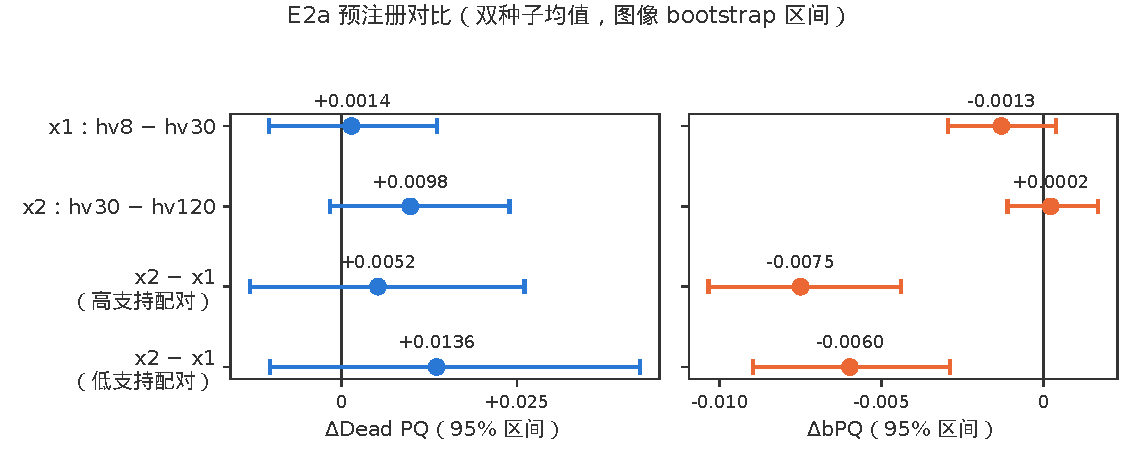
\includegraphics[width=\linewidth]{figs/e2a_contrasts_zh.pdf}
\caption{四项预注册比较的 Dead PQ、bPQ 差值及图像 bootstrap 区间。Dead 的四个区间均跨零；bPQ 的两个尺度比较区间均整体低于零。图中为双种子均值。}
\label{fig:e2a}
\end{figure}

这些结果支持以下判断\cite{hvres}：
\begin{enumerate}
\item \textbf{现有证据不支持用 x1 降门槛替代 x2。}Dead 差值在两个种子间一负一正（$-0.00138$ / $+0.00426$），bPQ 则均下降。x1\_hv8 的 strict Dead 均值虽较高，却没有同时满足官方 Dead 指标稳定改善和整体指标不下降的要求。
\item \textbf{x2 内降低门槛有正向信号，但尚不能认定为稳定改进。}hv30 相对 hv120 的官方 Dead PQ 在两个种子上均提高（$+0.01083$ / $+0.00880$），平均 $+0.00982$；但 bootstrap 区间跨零，且 seed 1 的 strict Dead 下降。
\item \textbf{按原图面积配平门槛后，x2 的 bPQ 损失仍存在。}两组尺度比较中，bPQ 的区间均完全低于零，两个种子的方向也一致。官方 Dead PQ 均值为正，但 strict Dead 在全部四个 x2$-$x1 种子配对中均为负，不能只报告前者。
\item \textbf{本轮没有完全解释尺度效应。}控制面积门槛后，采样、特征尺度和目标离散化仍随尺度变化。训练日程也尚未单独检验：编码器解冻时，学习率已衰减至 $5.16\times10^{-6}$。
\end{enumerate}

对象统计补充了指标所不能说明的细节。以同一批 741 个内部 Dead 核为分母，x1\_hv30 的匹配率为 61.27\%，x2\_hv120 为 70.99\%。因此，即使按原图面积配平门槛，x2 的内部 Dead 匹配率仍高出近 10 个百分点。相反，在 x2 内将门槛从 120 降到 30，内部匹配数的双种子均值仅从 526.0 变为 526.5，即两个种子合计只多匹配 1 个核。这表明 $+0.00982$ 的官方 Dead PQ 增益不能主要用“额外找回内部完整核”解释；掩码形状和误报分布也可能起作用，本轮尚未进一步分解。贴边 Dead 核的匹配率同样随尺度提高（40.21\%$\to$48.25\%），在 x2 内则几乎不受门槛影响。

\subsection{对后续实验的影响}

默认 \code{hv\_min\_size=30} 保持不变，x2\_hv30 保留为后续机制比较的固定参照。本轮结果不作为新的三划分测试收益发布。

DSB 的闸门 A 使用事先规定的点估计规则：x1 降门槛的 Dead 增益，与原 x2 相对 x1 的 Dead 增益之比为 $r/R=0.00144/0.01503=9.59\%$。它既未达到 50\% 的更换基线条件，也未达到 90\% 的降低架构路线优先级条件；x1\_hv8 同时还有 $-0.00130$ 的 bPQ 损失。因此，该闸门允许 DSB 继续使用 x1\_hv30 基线。\textbf{9.59\% 是用于执行预注册规则的比值，不是门槛所占因果贡献的估计。}DSB 是否最终启动训练，还取决于其余检验。

\section{DSB：训练 Dead 专家分支前的四项检验}

\subsection{设计思路与继续条件}

Dead 专家分支（DSB）基于两步假设：若 Dead 与常见类的优化目标在共享解码器上存在梯度冲突（H1），另设 Dead 检测分支便可能缓解冲突，在不损害整体指标的前提下找回内部漏检核（H2）。拟议模型保留原有编码器及 NP、HV、TP 三个分支，另加一组 NP+HV 专家分支；只在含 Dead 的图上计算专家损失，新增预测去重后再并入原结果。

方案没有沿用此前无效的平衡采样，也未采用正类权重 \code{pos\_weight}，而是通过损失掩码限定监督范围。原设计还担心大量纯负批次（约 97\%）对专家学习和 BatchNorm 统计的影响；但损失加权并不直接决定 BatchNorm 统计，损失掩蔽能否解决问题也未经过专家训练验证。文献核查未找到同时具备“类别解耦专家、细胞核实例分割、PanNuke 官方三划分、等参数量对照”的正面证据；作为设计参考的是分类领域的 GS-MoE 和半监督腺体分割的 Semi-MoE\cite{gsmoe,semimoe}，不能把它们的结果直接视为对本方案的支持。完整设计、预算及停止条件见预注册规格\cite{dsbspec}。

按规格 \S6，四项训练前检验全部满足条件，才进入开发训练；任一不满足，则停止本方案，保留机制分析。相关模型、目标、损失、TTA、命令行、合并选择、样例拼图和闸门脚本均已按测试驱动开发完成。代码在检验结束后合入 master，仅作为已测试工具保留，未用于专家分支训练。

\begin{table}[H]
\centering\small
\caption{四项预注册检验及其判定条件（规格 \S6 摘要）。“通过”表示可以继续检验本方案，不表示方法已经有效。}
\label{tab:gates}
\begin{tabularx}{\linewidth}{lYY}\toprule
闸门 & 检验内容 & 预注册判定条件\\\midrule
A & E2a 门槛比较 & x1 降门槛复现 $\geq$50\% 尺度 Dead 增益则更换基线；$\geq$90\% 且无性能代价则降低架构路线优先级\\
B & 梯度冲突探针 & Dead 组与常见类组梯度余弦为负的批次比例 $\geq$30\%，或逐层显著为负\\
C & L0 决策解耦上界 & 免训练的按类阈值/解码菜单若得 $\Delta$Dead $\geq$ $+0.005$ 且 bPQ 代价 $\leq$0.001，则停止本架构方案\\
D & Dead oracle 上界 & 内部漏检 Dead 以 IoU 0.7 oracle 加入后 $\Delta$Dead $\geq$ $+0.01$\\\bottomrule
\end{tabularx}
\end{table}

\subsection{A、C、D：允许继续检验}

\textbf{闸门 A：继续，保留 x1\_hv30 基线。}9.59\% 分别低于 50\% 和 90\% 的条件，故不更换基线、不降低该路线优先级。输入值经独立复算，与 E2a 冻结快照一致。

\textbf{闸门 C：继续。}在验证折 fold 2 上，比较 Dead 专属解码阈值 $\tau_{\mathrm{dead}}\in\{0.5,0.4,0.35,0.3\}$，其中 0.5 为基线。Dead PQ 从 0.16386 最高升至 0.16601（$\tau=0.4$），最大增益为 $+0.00214$，对应 $\Delta$bPQ 为 $+1.1\times10^{-5}$。它没有达到 $+0.005$ 的停止条件，因此该有限菜单不足以替代拟议的架构实验；这不等于证明所有决策层方法都无效。基线 Dead PQ 与官方评估完全一致；重解码路径的 mPQ、bPQ 基线有 $10^{-7}$ 量级差异，不能声称所有指标均逐位一致。

\textbf{闸门 D：通过。}把 fold 2 中全部 267 个未匹配的内部 Dead 真值，按 IoU 0.7 的收缩掩码补入基线预测，Dead PQ 从 0.16386 升至 0.31992，增量为 $+0.15606$；bPQ 增加 $0.00145$，mPQ 增加 $0.00231$。若直接使用精确真值掩码，Dead PQ 增量为 $+0.24533$。这类使用真值的理想化试验称为 oracle；它不是可部署方法，只用于估计“若能找回这些核，指标还有多大提升空间”。结果明显高于 $+0.01$ 的继续条件，支持把内部 Dead 漏检作为值得研究的问题，但不保证实际模型能够达到这一收益。

\subsection{B：首次测量无效，修正后未满足继续条件}

梯度探针在冻结的 split1 检查点上，将 Dead 像素和常见类像素分成互不重叠的两组。同一批数据做一次前向，分别对两组代理损失反向传播，再计算共享解码器参数的梯度余弦。余弦为正表示两组更新方向大体一致，为负表示相互冲突。预注册要求是负余弦批次占比至少 30\%，或逐层检验发现显著负值。

首次运行（10 月 8 日 00:58）被判为无效测量（VOID），不是闸门失败。原计划按顺序取 fold 1 的前 256 张图，结果全部来自 Breast 组织，只有 1 张含 Dead。64 批中有 63 批的 Dead 损失为零，却仍被计入冲突比例的分母；于是，无论唯一有效批的梯度如何，冲突比例最多也只有 1/64。该有效批的解码器复合余弦为 $+0.269$。核查确认，掩码划分、一次前向、\code{retain\_graph} 和参数集合没有问题，问题在取样方式及有效批次的定义。

修正方案先登记、再补充四个测试用例，经确认后重跑：按固定种子分层取样，覆盖全部 65 张 Dead 阳性图；分母只计 Dead 损失有效的批次；若 $n_{\mathrm{active}}<16$ 则判为 VOID；逐层比较采用单侧 $t$ 检验和 Holm 多重校正。重跑约使用数分钟 GPU 时间，这是探针测量，不是专家分支训练。

\begin{table}[H]
\centering\small
\caption{闸门 B 修正后的测量：覆盖 65 张 Dead 阳性图，64/64 批的 Dead 损失有效，每批 4 图。解码器复合余弦合并跳接、NP、HV、TP 四组参数计算。}
\label{tab:gateb}
\begin{tabular}{lrrr}\toprule
参数组 & 逐批余弦均值 & 负批次 & 冲突比例\\\midrule
编码器 & $+0.406$ & 0/64 & 0.000\\
跳接适配层 & $+0.608$ & 0/64 & 0.000\\
NP 分支 & $+0.917$ & 0/64 & 0.000\\
HV 分支 & $+0.760$ & 0/64 & 0.000\\
TP 分支 & $+0.196$ & 7/64 & 0.109\\
解码器复合 & $+0.749$ & 0/64 & 0.000\\\bottomrule
\end{tabular}
\end{table}

\begin{figure}[H]
\centering
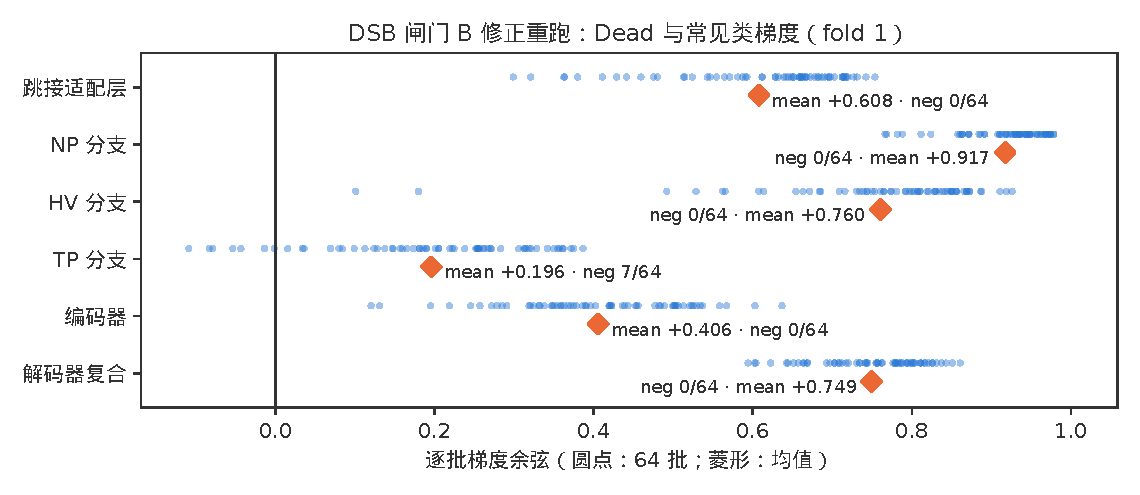
\includegraphics[width=\linewidth]{figs/gate_b_cosines_zh.pdf}
\caption{闸门 B 修正后的逐批梯度余弦分布。圆点为 64 个有效批次的取值，菱形为均值。解码器复合余弦全部为正；分组中仅 TP 分支出现 7 个负值。}
\label{fig:gateb}
\end{figure}

解码器复合余弦的均值为 $+0.749$，最小值 $+0.594$、中位数 $+0.760$、最大值 $+0.861$，\textbf{64 批中没有一批为负}，未达到 30\% 的继续条件。六个参数组的均值均为正，逐层单侧 $t$ 检验统计量也均为正（解码器复合 $t=+89.6$），没有经 Holm 校正后显著为负的组。因此，闸门 B 未通过。若假定批次独立、真实冲突率至少为 30\%，64 批全非负的概率约为 $10^{-10}$；但本次批次重复使用同一批图像，不能据此给出独立样本意义上的显著性结论。

这一结果有明确边界。探针测的是训练完成的基线检查点（回退检查点来自另一种子），使用按组计算的 NP-CE、TP-CE 和 HV-MSE 代理损失，而非完整训练目标。余弦只反映方向，不反映梯度幅度，也不覆盖早期训练动态。在这些条件下，Dead 与常见类的梯度大体同向，不支持预注册 H1 所要求的冲突证据；但不能由此推断整个训练历程从无冲突，更不能直接断言专家分支一定无效。

\subsection{按预注册规则停止 DSB}

按规格 \S10，任一闸门未通过便停止该方案，不增加训练预算。因此，DSB 的小规模试跑、开发轮和确认轮均未启动，配套的样例盲审与开发队列也未执行。\textbf{停止的是这项有明确前提的实验方案，专家分支是否有效（H2）从未被训练实验检验。}

四项检验共同缩小了下一步的范围：已测阈值菜单的收益只有约 $+0.002$，梯度探针未发现本方案要求的冲突，而理想化找回内部漏检核仍有 $+0.156$ 的提升空间。结合此前无效的重加权和平衡采样配方，现有证据不支持继续沿原 DSB 方案投入算力；但也不能排除所有损失设计、容量分配或数据方法。后续应先弄清候选核和标注中的不确定性，再决定是否研究新的检测监督或候选筛选方法。

\section{E0：两模型系统需要多少推理时间}

E0 采用固定计时流程：共享 A100-SXM4-80GB，批大小 32，解码使用 16 个进程，模型前向使用 bf16 自动混合精度（autocast）。沿用 \code{predict\_fold} 的推理流程，每 256 张图记录一块实际耗时。计时数据为 fold 2 的 2,523 张图，即所用 split2\_seed1 模型的训练折；没有读取测试折或计算性能指标。CPU 融合逐图重放冻结的 split2\_seed19 EF-P2 调用，新增实例数为 1,542，与冻结选择完全一致，确认计时使用的是对应的融合路径。

\begin{table}[H]
\centering\small
\caption{E0 在 10 月 8 日冻结的计时汇总，保留原分块等权均值及原重复选择结果；不是修正后的图像加权估计。融合为 CPU 单线程。10 月 9 日勘误见正文。}
\label{tab:e0}
\begin{tabular}{lrrrr}\toprule
环节 & ms/图 & 图/秒 & 峰值显存 (GiB) & 相对 x1\\\midrule
x1 & 15.50 & 64.4 & 4.76 & 1.00\\
x2-du2（GPU） & 52.88 & 18.9 & 12.91 & 3.41\\
x1-TTA（GPU） & 72.33 & 13.8 & 4.93 & 4.67\\
融合（CPU） & 25.97 & --- & --- & 1.68\\
两模型系统合计 & 94.35 & --- & --- & \textbf{6.09}\\\bottomrule
\end{tabular}
\end{table}

\begin{figure}[H]
\centering
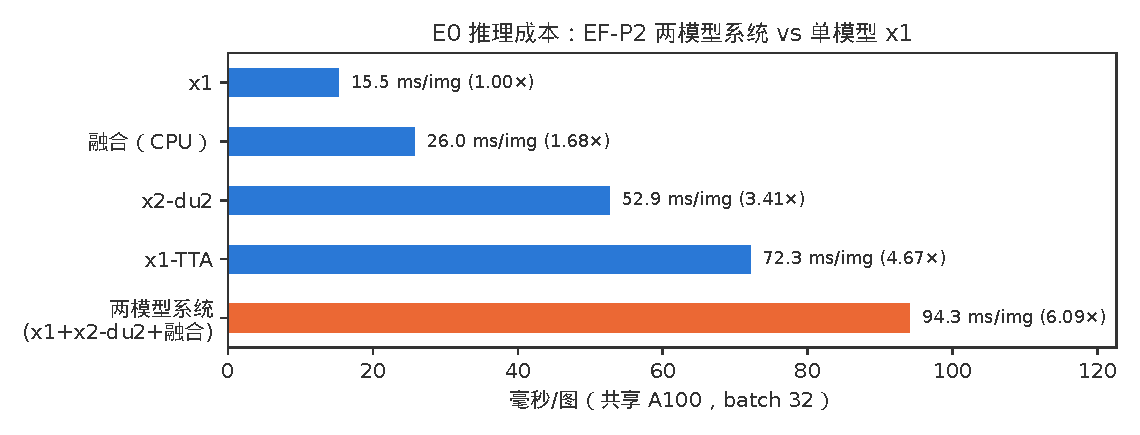
\includegraphics[width=\linewidth]{figs/e0_cost_zh.pdf}
\caption{保留 10 月 8 日冻结图：各环节的每图耗时及相对 x1 的倍数。两模型系统为 x1、x2-du2 与 CPU 融合之和；图像加权修正不改变约 6.1 倍的结论。}
\label{fig:e0}
\end{figure}

\textbf{10 月 9 日勘误。}旧汇总把不足 256 张的尾块与完整块等权平均。利用同一份 \code{cost.json} 保存的总吞吐量，按“每图平均毫秒 $=1000/\mathrm{img\_per\_s}$”恢复图像加权均值，并重新选择吞吐最高的一次重复，得到：x1 为 15.506464 ms/图，x2-du2 为 52.870378 ms/图，x1-TTA 为 72.309163 ms/图；CPU 融合仍为 25.971742 ms/图。两模型/x1 的比值由历史值 6.08687 修正为 \textbf{6.08447}，TTA/x1 由 4.66653 修正为 \textbf{4.66316}。这只是对同一测量的算术修正，不是新的 GPU 实验；旧表、旧图和冻结快照保留，便于追溯。

绝对耗时受同机负载影响。四次启动窗口的系统负载在 19--46 之间，x1 的平均耗时在 10.7--15.5 ms/图之间变化；所观察到的 x2/x1 比值为 3.1--3.4，两模型/x1 为 6.1--6.3。TTA 的波动更大，为 3.3--4.7。各配置不是同时测量，重复次数也不完全相同，因此这些比值是当前流程在所测窗口内的成本描述，而非可直接迁移到其他设备的延迟保证。

另有两点需要说明。旧产物中的 fp32 标签不准确，实际前向一直使用 bf16 autocast，本文已更正这一表述；分块计时的 p95 也不等于单张请求延迟的 p95。CPU 融合的最终计时使用一次性载入的数组，排除了逐实例反复解压 npz 带来的额外开销；首测曾因此达到每图 1--27 秒，旧记录和修正过程均保留。

按 E0 预注册规则，若不能证明性能收益足以抵偿成本，EF-P2 就不作为部署改进。现有 Dead PQ 收益较小，而两模型系统约需 x1 的 6.1 倍、x1-TTA 的 1.3 倍时间。因此，它更适合用于研究跨尺度互补，或作为后续教师模型的候选；教师模型能否带来有效蒸馏，尚未检验。M/S 后处理没有单独计时，模型加载、评测和融合并行化也未计入，本轮不能声称覆盖了全部端到端部署开销。

\section{文档、代码与实验产物的复核}

10 月 8 日的审计核对了文档与代码、报告数字与实验产物，以及运行记录，并执行了全量测试，当时为 \textbf{271 项通过}。10 月 9 日再次复核后，阶段三的 108 项指标差值、阶段四冻结快照及四道闸门判定均可重算，E0 的均值算法则按上一节修正。新增防护修复后的全量测试为 \textbf{277 项通过}。这些结果支持主要结论可复核，但不能概括为“全部历史产物都已重新验证”。

已完成的更正包括：CellViT-UNI 三划分 bPQ 由先舍入再平均的 0.6654，更正为按原始汇总精确平均的 \textbf{0.6653}；免训练找回方法的负结果改为“逐折最大回落 $-0.0012$”；KongNet 训练折 F1 间距改为 $\geq$0.12（最小 0.124）；跨域降幅记录中的 CellViT 0.152$\to$0.154 等。它们是按原始记录核对后的转录更正，不是新实验结果。

两个丢失的产物---fold 3 失败实例清单、split2\_seed2 的 du2/du2lev 测试评测---已从保留的确定性预测重建。重建值与历史记录一致：du2 为 0.48682/0.65836/0.15259，后处理增量为 $+0.00157$/$+0.00238$/$+0.00071$，对应网格判定不变；来源通过 SHA-256 校验记录绑定。开发与探针脚本也增加了 \code{fold\_guard} 检查，拒绝读取所属划分的测试折或无法核实划分号的输入；冻结评估菜单绑定输入哈希，不允许覆盖。

仍有两类复核缺口。CONCH 支柱 A 的部分探针输出没有留存缓存，无法从原输出重算。另在 10 月 9 日执行 P0--P3 完整来源检查时，旧清单与后来补齐种子的同名目录发生冲突，脚本按设计拒绝继续；没有修改旧清单或绕过检查使其“通过”。这不改变阶段三、四已核对的数字，但意味着历史 P0--P3 全量来源链仍待恢复。详细范围见 \code{docs/RESEARCH\_AUDIT\_2026-10-09.md}。

\section{局限与后续工作}

\subsection{本阶段的局限}

\begin{enumerate}
\item \textbf{E2a 只覆盖单划分、双种子。}全部比较在 split 1 的验证折上进行，bootstrap 只反映图像抽样不确定性；Dead 的四个区间均跨零，不能据此宣布稳定的三划分收益。
\item \textbf{梯度探针只覆盖训练完成的检查点和所选代理损失。}早期动态、完整训练目标和梯度幅度不在测量范围内，重复使用图像也限制了独立样本解释。
\item \textbf{专家分支的有效性未受检验。}DSB 在训练前停止，结论是没有满足该方案的继续条件，不是所有专家分支均无效。
\item \textbf{成本来自共享 GPU 上的分块计时。}各配置非同时测量，绝对耗时不能直接外推；M/S、模型加载、评测及并行融合没有全部纳入。
\item \textbf{本阶段没有新增三划分测试成绩。}验证折机制实验与历史测试产物审计分别报告；阶段三的测试折复用及统计限制仍然存在。
\end{enumerate}

\subsection{下一步先核实候选核，再决定训练路线}

截至本报告对应的实验阶段，优先事项仍是 E1 独立候选盲审\cite{next}。从验证数据中分别抽取 x1 接受的候选、x2 独有且被接受的候选、x2 独有但被拒绝的候选，以及随机背景区域，由独立评审判断其中是真实核、碎屑、边界或形状偏差，还是疑似漏标；允许保留“当前视野无法判断”的答案。目的不是把不匹配对象都解释成漏标，而是确定误报究竟由哪些情况组成。

若盲审表明新增核中有能够可靠筛选的有效对象，再考虑路线 B 的实例效用学习：训练数据内部交叉拟合，预测补入某个候选能否改善结果，并与冻结 EF-P2、低维回归和等算力的 TTA/集成作比较。$P(\mathrm{match})\cdot E[\mathrm{IoU}\mid\mathrm{match}]>q/2$ 仅是已有提案中的代理判据，须明确其假设，不能替代实际集合指标验证。路线 A 的裁剪一致性和路线 C 的跨模态监督继续作为有条件的备选，尚未获准启动。现有梯度探针、样例拼图和 oracle 工具可以复用，但工具就绪不代表新路线已得到验证。

\section{结论}

本阶段厘清了三个问题。第一，固定 HV 面积门槛确实使两种尺度的小核监督不同，但在本轮设置中，仅降低 x1 门槛不足以替代 x2；按原图面积配平后，x2 仍伴随官方 Dead PQ 均值上升与 bPQ 下降，strict Dead 则在四组配对中均下降。9.59\% 是预注册判定用的比值，不应解读为完整的因果分解。

第二，训练完成的基线检查点上，所测代理损失没有显示 DSB 预设的梯度冲突：64 批解码器复合余弦均值为 $+0.749$，没有负值。依照事先登记的规则，DSB 停止，专家分支未经训练，其有效性仍是未检验的问题。第三，两模型系统的推理时间约为 x1 的 6.1 倍，图像加权修正值为 6.08447；现有收益尚不足以支持部署优势，EF-P2 保留为机制研究与教师模型的候选。

主要结果已从冻结产物复核，成本汇总和历史转录错误已明确更正，未恢复的来源链也单独保留。下一步应先核实新增候选的真实性与可筛选性，再决定是否值得开展新的训练实验，而不是继续在已多轮观察的测试图上扩大筛选规则。

\appendix
\section{文件、数字与复现入口}

\subsection{数值核验}

10 月 8 日冻结的表格由 \code{scripts/report4\_numbers.py} 从实验产物输出。\code{scripts/verify\_report4.py} 使用 8 份审计评测 \code{summary.json}、五个闸门 JSON、\code{cost.json} 及审计涉及的测试汇总，独立重算并核对数字。本目录的 \code{verified\_numbers.json} 保留这一历史快照，其中 E2a 共核对 96 个指标单元：48 个单次训练指标、24 个配置均值、24 个比较均值。bootstrap 区间取自 E2a 冻结快照并记录来源 SHA-256，不重新抽样。闸门 B 的逐批余弦和各组 $t$ 值由保存的序列重算，闸门 A 比值与历史 E0 比值由原始记录重算。

10 月 9 日成本加权修正另存于 \code{docs/results/inference\_cost\_audit\_20261009.json}，不覆盖上述历史快照。研究日志\cite{findings}用于追溯过程，不代替原始产物作为数值依据。

2026 年 10 月 8 日全量回归测试为 271 项通过、64 条警告；10 月 9 日修复后的全量测试为 277 项通过、64 条警告。依赖环境为 Python 3.10、torch 2.5.1+cu124、numpy 1.23.5，未安装或升级依赖。图表沿用阶段报告三的中文字体与 Type 42 嵌入约定，其数值与 \code{figs/} 内冻结 CSV 一致；本次文字修订没有重新生成历史图表。

\subsection{产物与复现命令}

\begin{table}[H]
\centering\footnotesize
\caption{主要实验产物，均相对仓库根目录；\code{runs/} 下为本地产物，不随 Git 分发。}
\begin{tabularx}{\linewidth}{lY}\toprule
路径 & 本报告用途\\\midrule
\code{runs/hv\_threshold\_controls\_20261006/} & E2a 八次训练的配置、日志、原始评估及审计重推评估。\\
\code{runs/analysis/hv\_threshold\_controls\_20261006/} & E2a 冻结数字快照与 bootstrap。\\
\code{runs/analysis/dsb\_gates\_20261007/} & 四闸门 JSON 与台账；\code{gate\_b\_v2.json} 为闸门 B 的有效版本，首次无效测量另行保留。\\
\code{runs/analysis/inference\_cost\_20261008/} & E0 计时、命令与尝试日志。\\
\code{runs/analysis/report4\_numbers.txt} & 本报告逐表数字快照。\\\bottomrule
\end{tabularx}
\end{table}

在固定依赖环境、仓库根目录执行：
\begin{quote}\small
\texttt{python scripts/report4\_numbers.py}\\
\texttt{python scripts/verify\_report4.py}\\
\texttt{python scripts/make\_report\_figures4.py}\\
\texttt{python -m pytest -q}
\end{quote}
核验脚本在产物缺失或数值不一致时以错误状态退出，不修改实验产物。重跑历史评测须使用相应源码快照，或明确登记为新的复核，不得绕过来源检查。成本修正的独立算式和只读复现命令见 10 月 9 日审计文档。

\begin{thebibliography}{9}
\raggedright
\bibitem{reports} bdd26 项目. 阶段报告三：跨尺度候选筛选与面积过滤[R]. 2026-10-06. \code{docs/report/stage_report_3/}.
\bibitem{next} bdd26 项目. 研究复盘与下一阶段路线（2026-10-06）[R]. \code{docs/RESEARCH_NEXT_2026-10-06.md}.
\bibitem{hvplan} bdd26 项目. HV 门槛四臂对照预注册计划[R]. 2026-10-06. \code{docs/superpowers/plans/2026-10-06-hv-threshold-controls.md}.
\bibitem{hvres} bdd26 项目. HV 目标门槛对照：结果与机制分析[R]. 2026-10-07. \code{docs/HV_CONTROLS_RESULTS_2026-10-07.md}.
\bibitem{dsbspec} bdd26 项目. Dead 检测专家分支（DSB）设计规格与实现计划[R]. 2026-10-07. \code{docs/superpowers/specs/2026-10-07-dead-specialist-branch-design.md}; \code{docs/superpowers/plans/2026-10-07-dead-specialist-branch.md}.
\bibitem{findings} bdd26 项目. 实验日志：2026-10-06 至 10-08 条目[R]. \code{docs/findings.md}.
\bibitem{pannuke} GAMPER J, ALEMI KOOHBANANI N, BENES K, et al. PanNuke Dataset Extension, Insights and Baselines[EB/OL]. 2020[2026-10-06]. \url{https://arxiv.org/abs/2003.10778}.
\bibitem{uni} CHEN R J, DING T, LU M Y, et al. Towards a general-purpose foundation model for computational pathology[J]. Nature Medicine, 2024, 30(3): 850--862. DOI: \href{https://doi.org/10.1038/s41591-024-02857-3}{10.1038/s41591-024-02857-3}.
\bibitem{cellvit} H\"ORST F, REMPE M, HEINE L, et al. CellViT: Vision Transformers for precise cell segmentation and classification[J]. Medical Image Analysis, 2024, 94: 103143. DOI: \href{https://doi.org/10.1016/j.media.2024.103143}{10.1016/j.media.2024.103143}.
\bibitem{gsmoe} GS-MoE：generalist--specialist 分支恢复低患病率类（项目规格核查所用简记）[EB/OL]. arXiv:2609.18688, 2026[2026-10-07]. \url{https://arxiv.org/abs/2609.18688}.
\bibitem{semimoe} Semi-MoE：任务级专家的半监督分割（项目规格核查所用简记）[EB/OL]. arXiv:2509.13834, 2025[2026-10-07]. \url{https://arxiv.org/abs/2509.13834}.
\end{thebibliography}
\end{document}
